\chapter{Generating Training Data to Build Resource Estimators}
\label{GenerateData.ch}

Estimating execution time and resource requirements is challenging due to several influencing factors. As illustrated in Mind Map Figure~\ref{fig:Mindmap}, each application has a unique configuration that impacts memory usage and execution time. Changes in one or more parameters, as shown in Figure~\ref{fig:log_tracking} B, can significantly alter resource requirements. Users typically estimate their resource needs based on previous runs and often reuse the same allocations when re-executing jobs. However, modifying job parameters—such as increasing the number of epochs or adjusting the batch size in DNN training—requires revising resource allocations.

For instance, increasing the batch size demands more memory, potentially requiring a larger GPU node, which is costly and subject to longer queue wait times. Alternatively, offloading the job to a CPU can slow down execution. These patterns form what we refer to as the \textit{history of executions}, which contains records of past job executions across various hardware configurations.

This leads to critical questions:
\begin{itemize}
    \item How can we access execution history from diverse users and workloads?
    \item What key features should be extracted from data traces to build an accurate Resource Estimator?
\end{itemize}

\section{Challenges for Curating Resource Estimation Training Data}
The following section outlines the dataset-related challenges that must be addressed to train a machine learning-based resource estimator effectively.

\subsection{Availability of Execution History}

A well-documented execution history is crucial for training models to learn utilization patterns, including memory requirements, execution times, hardware allocations such as CPU, GPU, and memory, and application-specific parameters like DNN training data, optimization settings, and batch size. However, supercomputing centers often restrict access to workload data due to competition and client confidentiality concerns. While some publicly available datasets, such as the MIT Data Center Challenge Dataset and TPUGraphs, have been developed to analyze and estimate DNN workloads, they come with limitations.

The MIT dataset provides high-level job information, including the DNN model type and allocated resources, but the execution details such as batch size, input data, and optimization settings are stored as low-level time-series logs of approximately 5TB with limited metadata. Extracting meaningful insights from this dataset requires additional models to process execution data for memory and runtime prediction.

Similarly, the TPUGraphs dataset is based on open-source BERT and convolutional models profiled on Google TPUv4. It encodes model architectures using node features, with each node represented by 140 attributes and adjacency maps for optimization graphs. This dataset, which is about 6GB in size, is designed for Graph Neural Networks (GNNs) and provides a scalable approach for modeling tensor operations. While this allows new architectures to be incorporated into estimators, the dataset is restricted to TPUv4. Since OSC and TACC use GPUs and CPUs, we require a broader dataset that captures resource estimation across multiple architectures. Although models trained on TPUGraphs can predict fit time per training step, they cannot estimate the total resource requirements for SLURM job submissions. Additional models are needed to predict total wall time, making the generation of training datasets for profiling GPU and CPU jobs essential. To address this, we focus on efficiently generating execution traces for target applications, ensuring the process remains quick and cost-effective.

\subsection{Understanding and Capturing Resource-Specific Features for Machine Learning}

Different types of applications have varying resource demands. Compute-intensive workloads, such as deep neural network training, require high computational power and optimized execution pipelines. I/O-intensive workloads, such as processing large text datasets, depend on high disk bandwidth and fast data retrieval mechanisms. Memory-intensive applications, including training large-scale models like BERT, require significant RAM capacity and efficient memory management strategies. Each workload has distinct characteristics that impact execution, including application hyperparameters, hardware attributes like CPU and GPU frequency, number of cores, memory, and bandwidth, as well as concurrency settings such as cores per node and thread count.

Manually engineering these features requires a deep understanding of the tool or application, resource allocation methods, and predictive modeling techniques. Custom feature engineering for each workflow and hardware architecture is often complex, time-consuming, and inefficient. To overcome this challenge, we propose a framework that can automatically extract execution features from historical job logs. By incorporating a human-in-the-loop approach, users can define execution configurations specific to their domain or workload, ensuring that resource estimations remain accurate, adaptive, and scalable across diverse computing environments.

\section{Human-in-the-Loop Training Data Generation and Processing for Resource Estimation}

Generating training data for building estimators involves two key steps:  
\begin{itemize}
    \item Workload Execution and Profiling: Capturing profile dumps by executing workloads on targeted systems.  
    \item Data Processing for Model Training: Processing the profiled data and transforming it into training data for building machine learning models.  
\end{itemize}

\subsection{Workload Execution and Profiling}
To address these challenges, we introduce a human-in-the-loop \textit{generate} component that emulates training data based on user-defined configurations. These configurations are classified into scaled-down (SD) executions, which run at a smaller scale to quickly gather profiling data, and full-scale (FS) executions, which provide validation at production-level configurations. This approach ensures that training datasets are efficiently generated while balancing computational cost and execution speed.

To emulate and profile the identified features for the targeted applications, as described in Chapter~\ref{ref}, we leverage several third-party tools.

The \textbf{Cheetah Experiment Harness and Campaign Management System (Cheetah)} automates the execution of target applications under different system and application configurations. Each job's configuration is specified in a campaign file, which defines execution parameters. Cheetah’s runtime module, Savannah, processes metadata from these campaign files to generate execution configurations, referred to as \textit{experiments}, and runs them on the target systems. Every experiment is assigned a unique workspace endpoint, where it stores the execution script, configuration settings, experiment logs, profile traces, and outputs. Additionally, Cheetah includes a post-processing script that collects features from the workspace endpoint after each experiment.

To capture runtime performance metrics, we integrate \textbf{Tuning and Analysis Utilities (TAU)} within Cheetah. TAU provides detailed runtime profiling, helping analyze execution behavior. Specifically, we use the \texttt{-io} command-line argument to monitor port activity, memory-mapped I/O bandwidths, and maximum bytes read/written per execution. Additionally, we use \textbf{Pytools} to extract static profiling information, including processor cores, memory specifications, and other execution environment configurations.

For hardware-specific metrics, we incorporate \textbf{NVIDIA-SMI} to collect GPU performance data such as memory utilization, compute load, and power consumption. Similarly, \textbf{SLURM} is used to capture CPU-related job metrics, providing insights into CPU time allocation, memory usage, and resource contention.

Finally, \textbf{TAPIS} is employed to validate user access to systems listed in the CI Database and to ensure that profiling jobs are executed only on authorized endpoints. This guarantees security and compliance while enabling effective profiling across different computing environments.

\subsubsection{Execution Trace Generation Using the CODAR Framework}

This component leverages the \textbf{CODAR Framework} to generate training data by executing applications under both scaled-down (SD) and full-scale (FS) configurations. The end-user specifies application-specific hyperparameters, while the CI Database retrieves all accessible execution endpoints via TAPIS. Training data is collected from SD runs, which execute the application at a reduced scale, enabling rapid and diverse workload generation across different allocation configurations. Over time, FS data is incrementally incorporated to validate and test the framework against both familiar and novel feature values, ensuring robustness in execution predictions.

FS runs are configured to scale execution traces, allowing the model to generalize across different hardware and input configurations. By combining SD and FS executions, we create an adaptable and efficient data generation process for training ML-based resource estimators.

\subsubsection{Training Data Generation for Targeted Applications}

This section provides an overview of the methodology used to generate training data for a representative set of workloads for the selected applications outlined in \ref{problem.ch}.

\paragraph{Application-Centric Features for Training Data Generation}

Below is a summary of the application-specific features used in generating training data.

\begin{figure}[h]
    \centering
    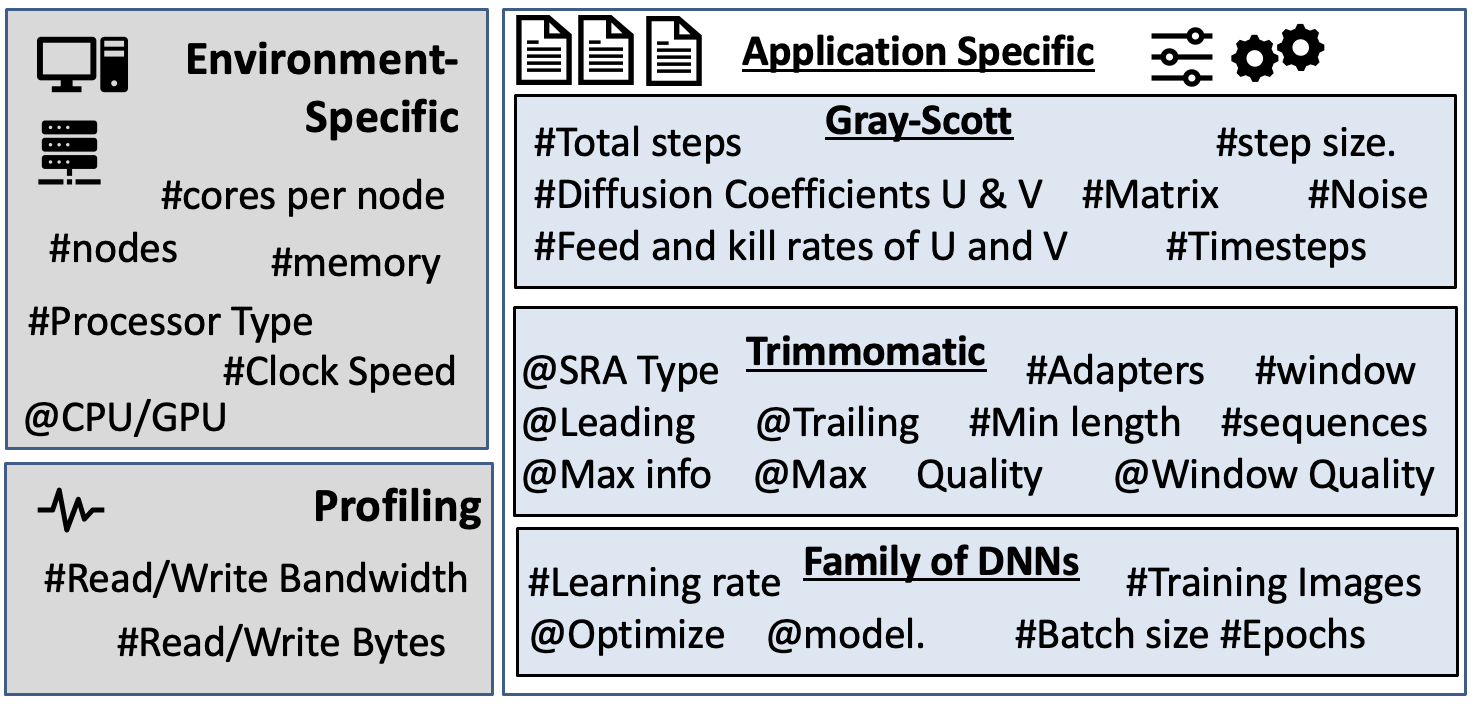
\includegraphics[width=0.9\textwidth]{Images/Features.png}
    \caption{Overview of environment-specific, application-specific, and profiling features used in resource estimation. \@ - Categorical Values and \#- Numeric values }
    \label{fig:features_overview}
\end{figure}


\begin{itemize}
    \item For the \textit{Gray-Scott} simulator, experiments were conducted by varying array dimensions, diffusion coefficients of the reacting chemicals, feed/kill rates, and the number of time steps. These simulations were executed across different environments with varying processor allocations. The scaled-down (SD) and full-scale (FS) runs differed in both array dimensions and the number of time steps.
    \item For \textit{Trimmomatic}, six different genome sequences were used as input short-reads. The trimming quality was influenced by parameters such as leading and trailing quality thresholds, minimum quality per window size, strictness, and minimum sequence length. Higher-quality genome sequences required less preprocessing time compared to lower-quality ones to achieve the same trim configurations. The SD and FS runs differed in genome sequence size, the number of processing threads, and execution environment configurations.
    \item For the \textit{family of DNNs}, three convolutional neural network (CNN) models were trained using different numbers of training samples and batch sizes. Experiments were conducted on both CPU and GPU nodes with varying core allocations, and execution times were measured based on the average epoch duration. The SD and FS runs differed in training sample count, batch size, number of epochs, and core allocation. FS runs were obtained by training the models on the entire dataset with larger batch sizes, utilizing all available cores of a single-node CPU or GPU HPC allocation.
\end{itemize}

Figure \ref{fig:features_overview} shows an overview of environment-specific, application-specific, and profiling features used in resource estimation. The environment-specific section captures hardware details such as cores per node and processor type. The application-specific section includes domain-dependent parameters for different workloads (Gray-Scott, Trimmomatic, and Family of DNNs). The profiling section captures read/write bandwidth and byte-level I/O operations.




\subsubsection{Understanding the Characteristics of Scaled-Down and Full-Scale Data}

\begin{figure}[h]
    \centering
    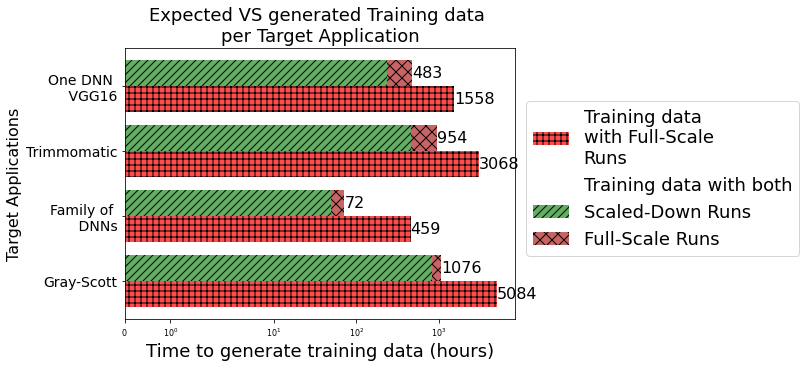
\includegraphics[width=0.7\textwidth]{Images/Cost_Graph.png}
    \caption{Distribution of training data generated using full-scale runs (FS) and scaled-down runs (SD).}
    \label{fig:cost_scaling}
\end{figure}

Executing resource-intensive applications on shared, production research cyberinfrastructures (CI) to generate large amounts of training data is expensive in terms of resources, cost, and time, especially when the application context keeps changing, necessitating the regeneration of training data. To reduce the cost of data generation, we studied the feasibility of generating training samples on commodity environments like workstations or low-contention resources such as single-node allocations.
To minimize execution time, we limited input configurations and application features that influence execution time. For example, in DNN training, we reduced the number of images in the training data, creating what we term "scaled-down" (SD) runs. Additionally, we executed the target applications at full-scale (FS) on each new CI for a few iterations to capture CI-specific characteristics in training samples.
We profiled the targeted application across a pre-identified set of configurations for both SD and FS runs. The SD executions covered a broader range of feature distributions and were repeated multiple times to exclude errors, while the FS executions focused on capturing CI-specific behaviors.
Graph \ref{fig:cost_scaling} presents the estimated cost of generating the entire training dataset using only FS configurations versus the actual cost of generating a combined dataset of SD and FS runs.

\begin{figure}[h]
    \centering
    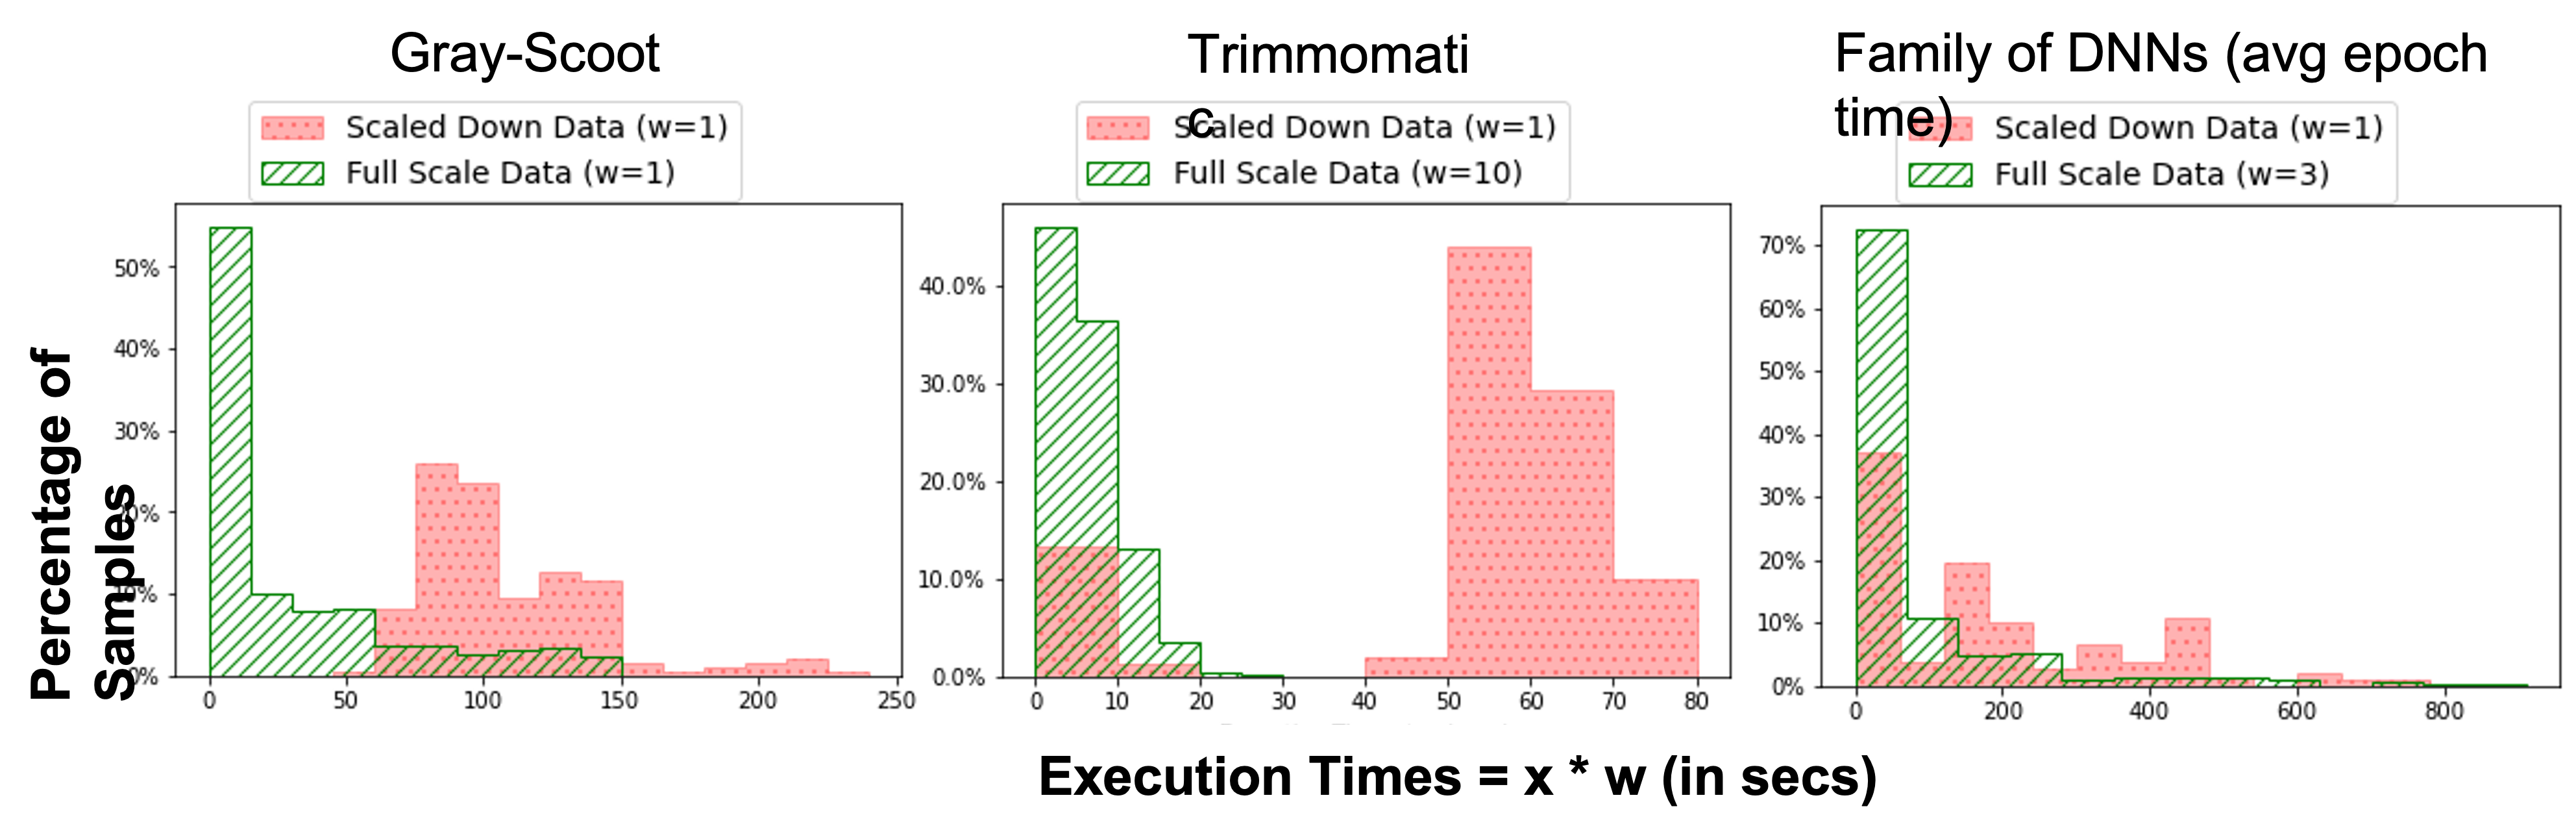
\includegraphics[width=0.95\textwidth]{Images/distribution_graph.png}
    \caption{Distribution of execution times across different workflows (Gray-Scott, Family of DNNs, and Trimmomatic)}
    \label{fig:execution_time_distribution}
\end{figure}

Figure \ref{fig:execution_time_distribution} illustrates the distribution of FS and SD samples generated across these three workflows.



\begin{table}[]
\caption{Characteristics of different combinations of ``scaled-down'' and ``full-scale'' generated samples when used as training and test sets. }
\label{tab:dataconfig}
\begin{tabular}{ccc}
\hline
\multicolumn{1}{|c|}{\textbf{}} & \multicolumn{2}{c|}{\textbf{Train \& Test}} \\ \hline
\multicolumn{1}{|c|}{\textbf{}} & \multicolumn{1}{c|}{\textbf{FS \& FS}} & \multicolumn{1}{c|}{\textbf{SD \& SD}} \\ \hline
\multicolumn{1}{|c|}{\textbf{\begin{tabular}[c]{@{}c@{}}No pre-processing - \\ ``Raw"Generated \\ Training Datasets\end{tabular}}} & \multicolumn{1}{c|}{\begin{tabular}[c]{@{}c@{}}-limited training data\\ -multicollinearity exists\\ - limited distribution of \\ samples over feature space\end{tabular}} & \multicolumn{1}{c|}{\begin{tabular}[c]{@{}c@{}}-no feature standardization\\ -multicollinearity exists\end{tabular}} \\ \hline
\multicolumn{1}{|c|}{\textbf{\begin{tabular}[c]{@{}c@{}}Features as\\ Principle Components\end{tabular}}} & \multicolumn{1}{c|}{\begin{tabular}[c]{@{}c@{}}-limited training data\\ - limited distribution of \\ samples over feature space\end{tabular}} & \multicolumn{1}{c|}{\textbf{\begin{tabular}[c]{@{}c@{}}IDEAL$^{\mathrm{b}}$ \\ Training and \\ Test Data\end{tabular}}} \\ \hline
\multicolumn{1}{|c|}{\textbf{\begin{tabular}[c]{@{}c@{}}Principle Components \\ + \\ Training Data Outliers\end{tabular}}} & \multicolumn{1}{c|}{\begin{tabular}[c]{@{}c@{}}-limited training data\\ -outliers exist\\ - limited distribution of \\ samples over feature space\end{tabular}} & \multicolumn{1}{c|}{-outliers exist} \\ \hline
\multicolumn{1}{l|}{} & \multicolumn{1}{c|}{\textbf{SD \& FS}} & \multicolumn{1}{c|}{\textbf{SD+n\%FS \& FS$^{\mathrm{a}}$}} \\ \hline
\multicolumn{1}{|c|}{\textbf{\begin{tabular}[c]{@{}c@{}}No pre-processing - \\ ``Raw"Generated \\ Training Datasets\end{tabular}}} & \multicolumn{1}{c|}{\begin{tabular}[c]{@{}c@{}}-unseen data\\ -no feature standardization \\ - multicollinearity exists\\ -training and test have \\ different distribution\end{tabular}} & \multicolumn{1}{c|}{\begin{tabular}[c]{@{}c@{}}-still has unseen data\\ -no feature standardization \\ -multicollinearity exists\\ -imbalanced SD and FS training\\ -training and test have \\ different distribution\end{tabular}} \\ \hline
\multicolumn{1}{|c|}{\textbf{\begin{tabular}[c]{@{}c@{}}Features as\\ Principle Components\end{tabular}}} & \multicolumn{1}{c|}{\begin{tabular}[c]{@{}c@{}}-unseen data\\ -training and test have \\ different distribution\end{tabular}} & \multicolumn{1}{c|}{\begin{tabular}[c]{@{}c@{}}-still has unseen data\\ -imbalanced SD and FS training\\ -training and test data have \\ different distribution\end{tabular}} \\ \hline
\multicolumn{1}{|c|}{\textbf{\begin{tabular}[c]{@{}c@{}}Principle Components \\ + \\ Training Data Outliers\end{tabular}}} & \multicolumn{1}{c|}{\begin{tabular}[c]{@{}c@{}}-unseen data\\ -outliers exist\\ -training and test have \\ different distribution\end{tabular}} & \multicolumn{1}{c|}{\begin{tabular}[c]{@{}c@{}}-still has unseen data\\ -outliers exist\\ -imbalanced SD and FS training\\ training and test data have \\ different distribution\end{tabular}} \\ \hline
\multicolumn{3}{l}{\begin{tabular}[c]{@{}l@{}}$^{\mathrm{a}}$ This is the training data generated through our pipeline, and \\ we want to train highly accurate regression models on this.\\ $^{\mathrm{b}}$ The ideal characteristics for training data. \\ We process the training data intending to achieve some of their characteristics.\\ SD and FS samples have different distributions for some environment-specific \\ features and input-features. \\ SD data represents ``huge'' training data with good sample space. \\ FS data has ``limited'' sample distributions over feature-space.\end{tabular}}
\end{tabular}
\end{table}

Table \ref{tab:dataconfig} presents the configurations and characteristics of scaled-down (SD) and full-scale (FS) runs used for training and testing datasets in different combinations. 
Some observed characteristics of SD and FS samples based on how training, validation, and test data are curated present several challenges:
\begin{itemize}
    \item In an ideal scenario, if the inference/test data follows the same distribution as the training data (IDEAL$^{\mathrm{b}}$ from Table X), the estimation error should remain minimal, regardless of the model used (see Table X in Chapter Y). However, due to the high cost of generating full-scale (FS) training samples, we cannot produce enough FS data to match the distribution of scaled-down (SD) executions. Using just SD data as training would lead to more scalability errors as the FS test data had “unseen” distribution. Training estimators using only FS samples fails to handle outliers and generalize across diverse workloads effectively.
    \item Additionally, \textbf{multicollinearity} becomes a challenge when two or more independent variables are highly correlated, making it difficult to distinguish their individual impact on the target variable. For example, training sample size and batch size are often strongly correlated, leading to unstable regression coefficients. As the number of identified features increases, the need for more training data grows, creating feature space expansion issues. Without proper f\textbf{eature selection or dimensionality reduction}, this can lead to overfitting and increased computational costs.
    \item Finally, \textbf{scalability} issues arise when transitioning from SD training to FS models, as the limited number of FS samples introduces a severe class imbalance. This imbalance skews model learning, reducing its ability to generalize effectively to unseen workloads. Addressing these challenges requires careful data sampling, feature engineering, and regularization techniques to balance SD and FS training distributions.
\end{itemize}




\subsection{Data Processing for Model Training}

To address these challenges, we explore \textbf{data preprocessing techniques} and the creation of effective train-test-validation splits to optimize the use of emulated training data:
\begin{itemize}
    \item Training Split: 100\% SD + n\% FS; Validation Split: n\% FS; Test Split: n\% FS - Incorporating a small percentage of FS samples into SD data for training enables regression models to scale predictions effectively when executed correctly. The validation dataset helps determine the appropriate scaling factor by minimizing errors, as it shares the same distribution as the test dataset (FS data) for every regression prediction model. However, excessive inclusion of FS samples in a predominantly SD training set may introduce outlier effects, impacting FS run observations.
    \item To tackle scalability issues and class imbalance, regularization techniques alone may limit the model's ability to learn generalizable scalability patterns from FS data. Sampling methods, such as \textbf{upsampling} FS data within the training set, help align training and test distributions, thereby reducing class imbalance and enhancing model robustness.
    \item To address multicollinearity, feature selection techniques remove redundant variables, while dimensionality reduction approaches, such as \textbf{Principal Component Analysis} (PCA) or feature extraction, retain essential information while reducing complexity. Regularization techniques, such as Ridge Regression (L2 regularization), further mitigate multicollinearity by penalizing large coefficients, improving model stability.

\end{itemize}

The pipeline "Building Regression Models" in figure \ref{fig:HARP_pipeline} illustrates a general machine learning workflow. Steps 1 and 2 cover the pre-processing methods described above, while Steps 3, 4, and 5 are detailed in the model development chapter (Chapter \ref{BuildEstimator.ch}).





